\documentclass[12pt, letterpaper]{article}

\usepackage{amsmath, amssymb}
\usepackage{physics}
\usepackage[french]{babel}
\usepackage[margin=2.5cm]{geometry}
\usepackage[utf8]{inputenc}
\usepackage[T1]{fontenc}
\usepackage{hyperref}
\usepackage{caption}
\usepackage{graphicx}

\begin{document}

\title{Devoir 3 : Équation de Schrödinger en dimension 1}
\author{PHQ404}
\date{Date de complétion suggérée : 23 mars 2024 à 23h45}
\maketitle

\section{Objectif}\label{sec:objectif}

\noindent L’objectif de ce TP est de se familiariser avec deux techniques pour solutionner des problèmes aux limites
en dimension 1 : la méthode du tir et la méthode des éléments finis.
Ces méthodes sont présentées au chapitre 12 des notes de David Sénéchal.


\section{Comment présenter et remettre votre TP}\label{sec:comment-presenter-et-remettre-votre-tp}

\noindent Vous devez cloner le répertoire github dans l'organisation du cours au lien suivant :\\
\href{https://classroom.github.com/a/eH84M6i-}{https://classroom.github.com/a/eH84M6i-}.
Dans ce répertoire se trouvera votre code python, vos tests unitaires ainsi que votre rapport
décrivant les méthodes utilisés et l'analyse de vos résultats.
La structure des fichiers ne doit pas être modifiée, mais vous pouvez ajouter des fichiers si vous le désirez.
Voici la structure de fichiers que votre répertoire devra garder :

\bigskip

\noindent Root
\begin{itemize}
    \item[]
        \begin{itemize}
            \item[$\rightarrow$] src
                \begin{itemize}
                    \item[$\hookrightarrow$] \texttt{fichier0.py}
                    \item[$\hookrightarrow$] \texttt{fichier1.py}
                    \item[$\hookrightarrow$] \dots
              \end{itemize}
        \end{itemize}
  \item[]
  \begin{itemize}
    \item[$\rightarrow$] tests
    \begin{itemize}
      \item[$\hookrightarrow$] \texttt{test\_fichier0.py}
      \item[$\hookrightarrow$] \texttt{test\_fichier1.py}
      \item[$\hookrightarrow$] \dots
    \end{itemize}
  \end{itemize}
  \item[$\hookrightarrow$] \texttt{.gitignore}
  \item[$\hookrightarrow$] \texttt{requirements.txt}
  \item[$\hookrightarrow$] \texttt{README.md}
  \item[$\hookrightarrow$] \texttt{rapport\_devoir\emph{i}-\emph{vos\_noms}.pdf}
\end{itemize}

\bigskip

\noindent Le fichier \texttt{requirements.txt} doit contenir les dépendances de votre projet.
Le fichier \\\texttt{README.md} doit contenir les instructions pour installer et utiliser votre projet ainsi
qu'une brève description du devoir et des méthodes utilisés dans le code.
Le fichier \\\texttt{rapport\_devoir\emph{i}-\emph{vos\_noms}.pdf} doit contenir votre rapport en format pdf.
L'utilisation de \LaTeX\ est fortement recommandée pour la rédaction de votre rapport.
Dans le dossier \texttt{src} se trouvera votre code python et dans le dossier \texttt{tests} se trouvera vos tests
unitaires.

\bigskip

\noindent La remise du code se fera à chaque \texttt{push} sur le répertoire github.
Notez que seul le dernier \texttt{push} sera considéré pour la correction.


\section{Énoncé}\label{sec:enonce}
\subsection{Méthode du tir}\label{subsec:methode-du-tir}

\noindent On considère l’équation de Schrödinger indépendante du temps pour une particule de masse unité dans
un potentiel quadratique
\begin{equation}
    \label{eq:schrodinger}
    - \frac{1}{2} \ddot{\psi} + \frac{1}{2} x^2 \psi = E \psi.
\end{equation}

\noindent On cherche les solutions pour $x$ de $-L$ à $L$ pour $L = 5$ avec 200 points
avec les valeurs initiales $\psi(-L) = 0$ et $\dot \psi(-L) = 0.001$.
La valeur initiale de $\dot \psi$ n'est pas très importante,
mais celle-ci devrait vous donnez une échelle raisonnable.
Vous devez :
\begin{itemize}
    \item
    Implémenter une fonction qui évalue $\psi(x = L|E)$ comme définie dans les notes.

    \item
    Implémenter une fonction pour cadrer une racine.
    C’est-à-dire, une fonction qui à partir d’une valeur $x_0$ et d’une fonction $f$,
    trouve une valeur $x_1$ telle que $f(x_1) = -f(x_0)$.
    Pour ce faire, on augmente $x$ par pas de $\Delta$ jusqu’à trouver
    $x_1$ ou atteindre un nombre limite de pas (20 par exemple).

    \item
    Trouver les racines de $\psi(x = L|E)$ à l’aide de l’algorithme de Brent et de la fonction précédente.

    \item
    À l’aide de ces fonctions, écrivez un programme qui trouve les 6 premières solutions à l’équation de
    Schrödinger (les 6 énergies les plus basses) et portez-les sur un même graphique en les décalant par la
    valeur de leur énergie, comme illustré à la figure~\ref{fig:exemple}.
\end{itemize}

\begin{figure}[h!!]
    \centering
    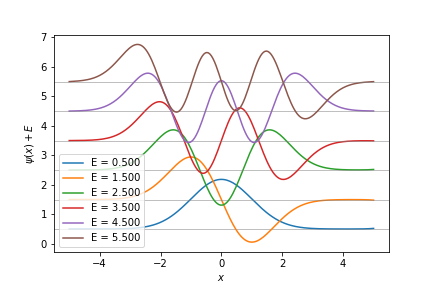
\includegraphics[scale=0.5]{../images/exemple}
    \caption{Exemple de figure pour les états propres de basses énergies
    de l'équation \ref{eq:schrodinger}.}
    \label{fig:exemple}
\end{figure}

\subsection{Méthode des éléments finis}\label{subsec:methode-des-elements-finis}

\noindent Dans cette partie, la méthode des éléments finis sera utilisée.
La méthode n’a pas besoin d’être programmée entièrement~:~un fichier python est fourni
et doit être importé dans votre programme.
Ce fichier introduit une classe pour vous aider.
Appliquez la méthode des éléments finis à la solution de la même équation qu’à la partie précédente.
Cette fois, utilisez une grille de 500 points et une borne $L = 6$.
Produisez le même type de graphique.
Idéalement, vous utiliseriez la même fonction pour le graphique que pour l'énoncé précédent.
Les fonctions de la classe ne calculent pas les valeurs aux frontières.
Celles-ci ne sont nécessaire et peuvent ajouter du bruit à vos solutions.

\bigskip

\noindent Note: Toutes les fonctions qui doivent être implémentées sont déjà définies dans les fichiers
et retournent des \texttt{NotImplementedError}.


\section{Vérification}\label{sec:verification}

\noindent Il est important de vérifer vos implémentations.
En effet, vous devez vous assurer que vos méthodes fonctionnent correctement et pour ce faire, vous devez rouler et
implémenter des tests unitaires qui testent chacune de vos classes et fonctions.
De plus, vous devriez tester si les résultats obtenus sont logiques.
Il serait aussi intéressant de retrouver vos vérifications dans votre rapport.
Il faut ajouter des tests unitaires dans le dossier \texttt{tests} afin d'augmenter la couverture des tests,
mais les tests déjà implémentés ne doivent pas être modifiés.


\section{Critères d'évaluation}\label{sec:criteres-d'evaluation}

\begin{description}
  \item[70 points] Pour le résultat obtenue à l'aide du module TAC\@.
  \item[30 points] Pour la qualité du rapport.
\end{description}


\end{document}
